% definit le type de document et ses options
\documentclass[a4paper,11pt]{article}

% des paquetages indispensables, qui ajoutent des fonctionnalites
\usepackage[latin1]{inputenc}
\usepackage[T1]{fontenc}
\usepackage{amsmath,amssymb}
\usepackage{fullpage}
\usepackage{graphicx}
\usepackage{url}
\usepackage{xspace}
\usepackage[francais]{babel}
% pour ecrire les reponses
\newtheorem{exercice}{Exercice}

% des commandes utiles pour ecrire des maths : rajoutez les votres!
\newcommand{\dx}{\,dx}
\newcommand{\ito}{,\dotsc,}
\newcommand{\R}{\mathbb{R}}
\newcommand{\N}{\mathbb{N}}
\newcommand{\Poly}[1]{\mathcal{P}_{#1}}
\newcommand{\abs}[1]{\left\lvert#1\right\rvert}
\newcommand{\norm}[1]{\left\lVert#1\right\rVert}
\newcommand{\pars}[1]{\left(#1\right)}
\newcommand{\bigpars}[1]{\bigl(#1\bigr)}
\newcommand{\set}[1]{\left\{#1\right\}}

% titre, auteur et date
\title{TP Principes et M\'{e}thodes Statistiques}
\author{Gabriel Sarrazin, Nejmeddine Douma, Simon Rabourg}
\date{Avril 2015}

% le debut du contenu
%===============
\begin{document}
%===============

% pour afficher titre, auteur et date
\maketitle



\section{Introduction}

TODO

\section{Analyse des défauts de cuves}

\begin{enumerate}

\item Les mesures des trois cuves présentent des valeurs minimums assez proches les unes des autres: 2.007, 2.006 et 2.059. La cuve 2 possède la valeur maximale 5.437 et la variance la plus grande 0.54127686. Tandis que la cuve 1 s'empare du maximum des écat-types 1.023202 et du maximum du coefficient de variation empirique 0.3563262. Les mesures de la cuve 3 présentent le plus de régularité avec le minimum de variation 0.15907528, le minimum d'écart-type 0.4163554 et de coefficient de variation empirique 0.1475989 .

D'après les allures des histogrammes des mesures de la cuve 1 (figures 1 et 2) et celles des mesures de la cuve 2 (figures 3 et 4), ces deux échantillions sont vraisemblablement de loi exponentielle. Les figures 5 et 6 montrent que les mesures de la cuve 3 sont vraisemblalement de loi normale.

\begin{figure*}[t]
\centering
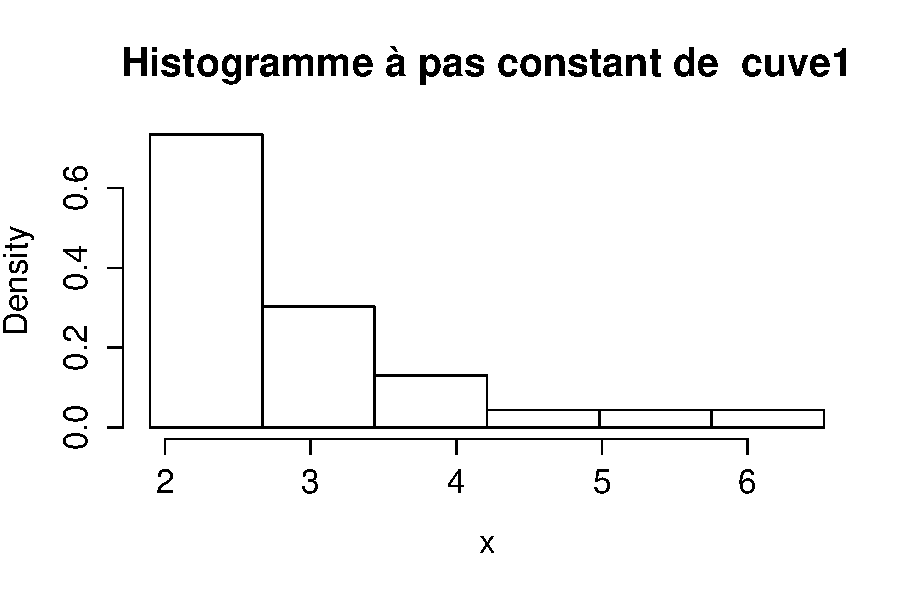
\includegraphics[width=1.0\textwidth]{figures/histopas_cuve1.pdf}
\caption{Histogramme à pas constant de cuve1 obtenu dans R}
\end{figure*}

\begin{figure*}[t]
\centering
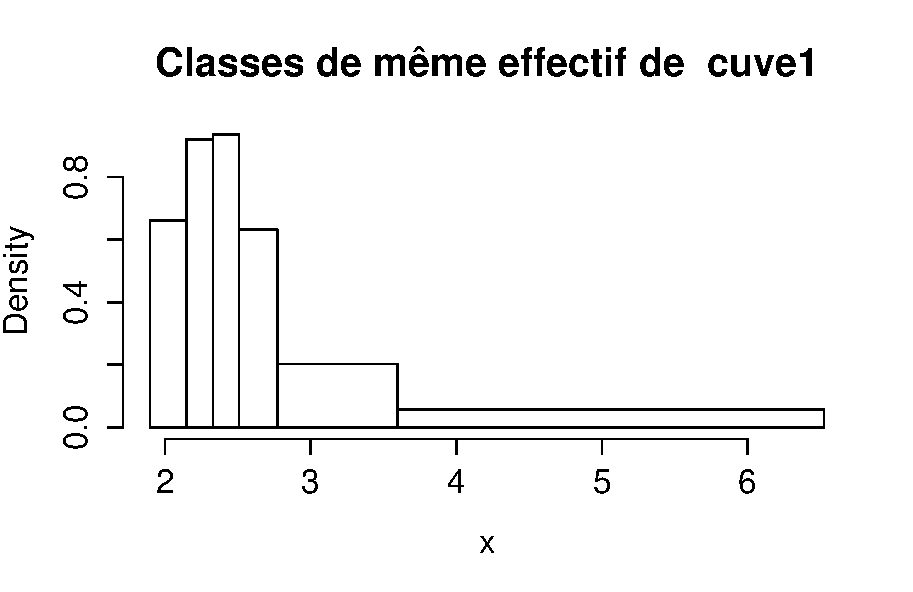
\includegraphics[width=1.0\textwidth]{figures/histoeff_cuve1.pdf}
\caption{Histogramme à classe de même effectif de cuve1 obtenu dans R}
\end{figure*}

\begin{figure*}[t]
\centering
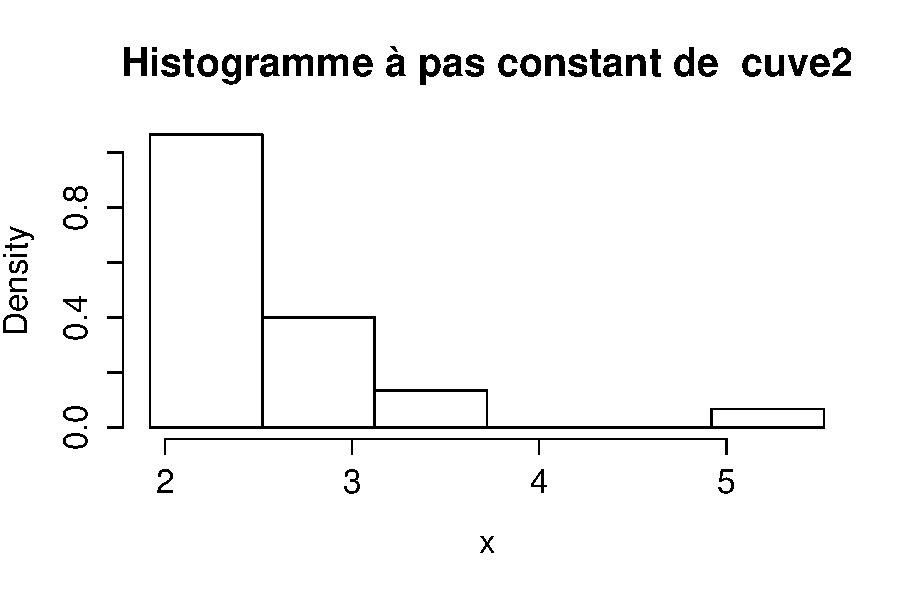
\includegraphics[width=1.0\textwidth]{figures/histopas_cuve2.pdf}
\caption{Histogramme à pas constant de cuve2 obtenu dans R}
\end{figure*}

\begin{figure*}[t]
\centering
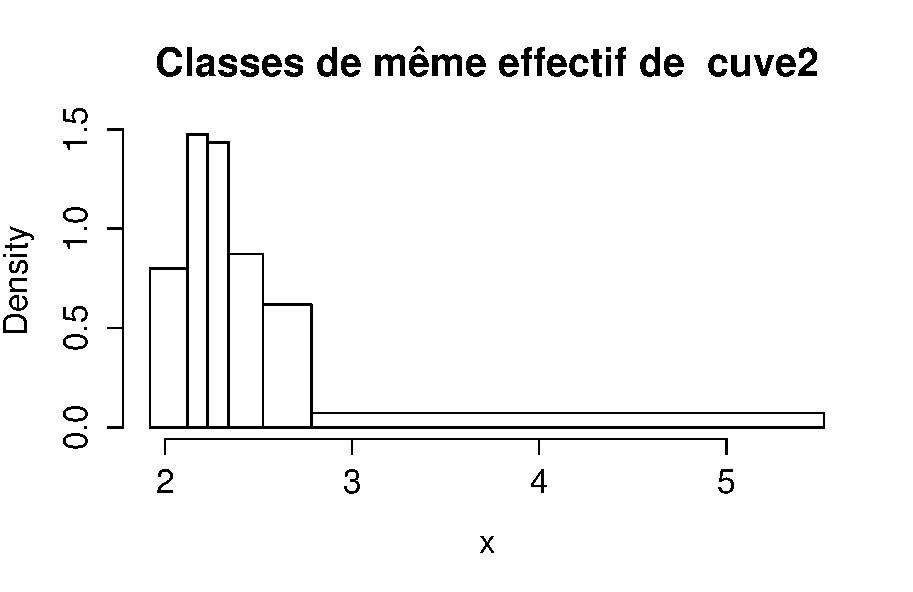
\includegraphics[width=1.0\textwidth]{figures/histoeff_cuve2.pdf}
\caption{Histogramme à classe de même effectif de cuve2 obtenu dans R}
\end{figure*}

\begin{figure*}[t]
\centering
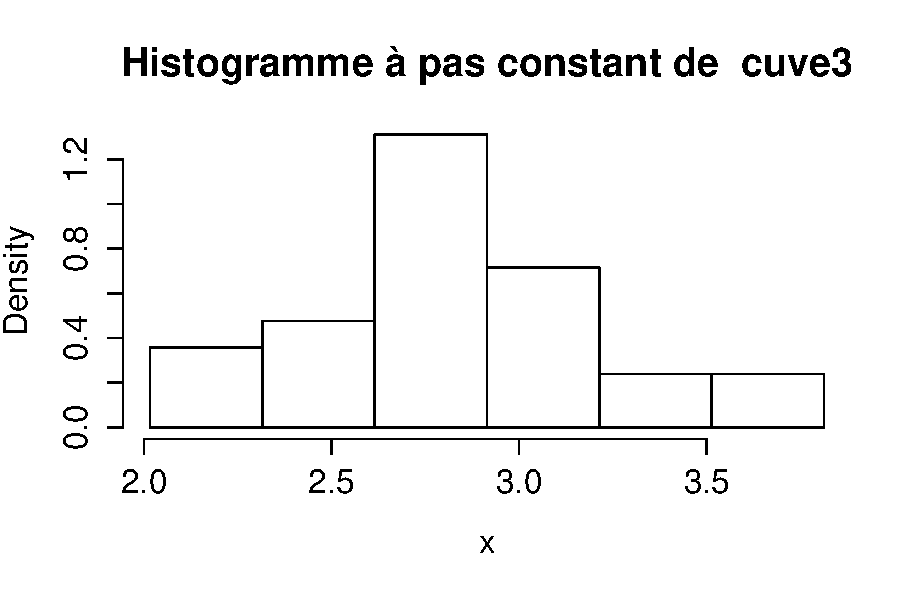
\includegraphics[width=1.0\textwidth]{figures/histopas_cuve3.pdf}
\caption{Histogramme à pas constant de cuve3 obtenu dans R}
\end{figure*}

\begin{figure*}[t]
\centering
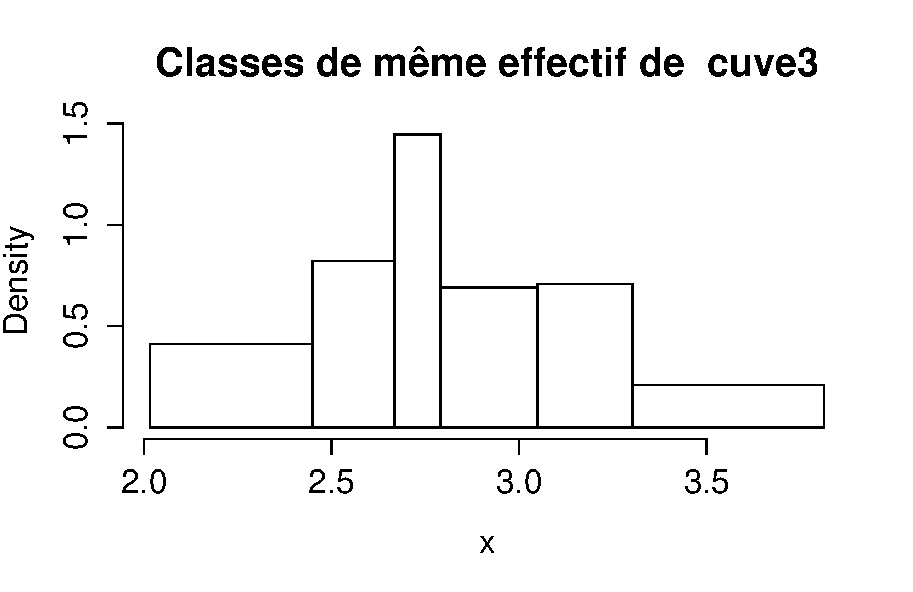
\includegraphics[width=1.0\textwidth]{figures/histoeff_cuve3.pdf}
\caption{Histogramme à classe de même effectif de cuve3 obtenu dans R}
\end{figure*}


\end{enumerate}






% fin du document
%=============
\end{document}
%=============
